\documentclass{standalone}
\usepackage{tikz}
\usetikzlibrary{patterns, positioning}

\begin{document}
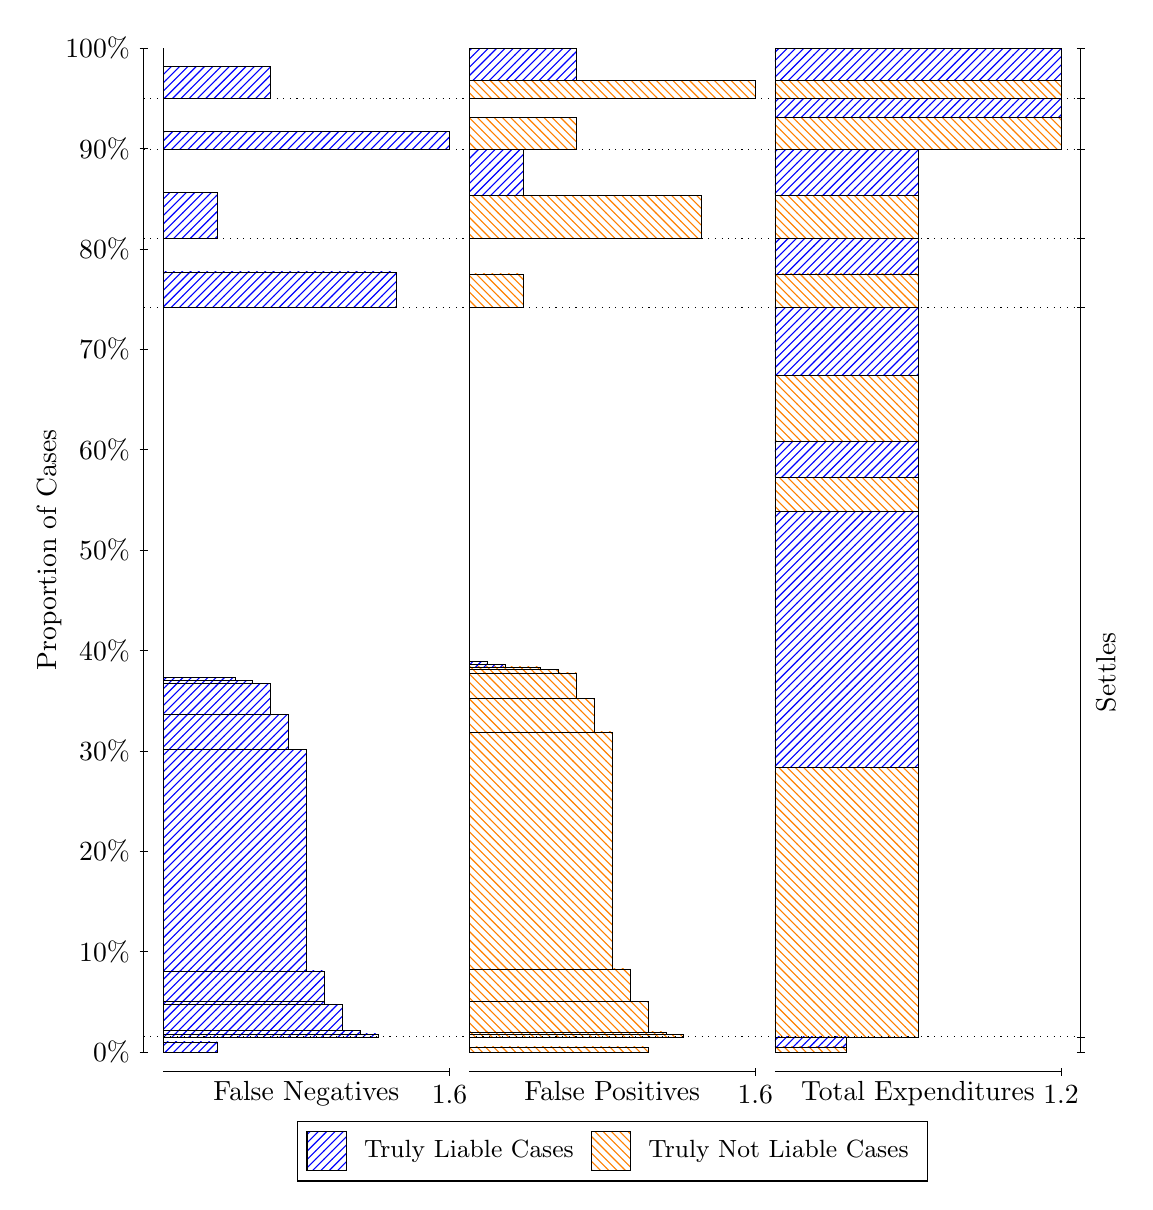
\begin{tikzpicture}
\draw[black, very thin] (1.5,1.75) -- (1.5,14.5);
\node[rotate=90, anchor=center] at (0.3, 8.125) {Proportion of Cases};
\draw[black, very thin] (1.45,1.75) -- (1.55,1.75);
\node[anchor=east] at (1.45, 1.75) {0\%};
\draw[black, very thin] (1.45,3.025) -- (1.55,3.025);
\node[anchor=east] at (1.45, 3.025) {10\%};
\draw[black, very thin] (1.45,4.3) -- (1.55,4.3);
\node[anchor=east] at (1.45, 4.3) {20\%};
\draw[black, very thin] (1.45,5.575) -- (1.55,5.575);
\node[anchor=east] at (1.45, 5.575) {30\%};
\draw[black, very thin] (1.45,6.85) -- (1.55,6.85);
\node[anchor=east] at (1.45, 6.85) {40\%};
\draw[black, very thin] (1.45,8.125) -- (1.55,8.125);
\node[anchor=east] at (1.45, 8.125) {50\%};
\draw[black, very thin] (1.45,9.4) -- (1.55,9.4);
\node[anchor=east] at (1.45, 9.4) {60\%};
\draw[black, very thin] (1.45,10.675) -- (1.55,10.675);
\node[anchor=east] at (1.45, 10.675) {70\%};
\draw[black, very thin] (1.45,11.95) -- (1.55,11.95);
\node[anchor=east] at (1.45, 11.95) {80\%};
\draw[black, very thin] (1.45,13.225) -- (1.55,13.225);
\node[anchor=east] at (1.45, 13.225) {90\%};
\draw[black, very thin] (1.45,14.5) -- (1.55,14.5);
\node[anchor=east] at (1.45, 14.5) {100\%};

\draw[black, very thin] (13.4,1.75) -- (13.4,14.5);
\draw[black, very thin] (13.35,1.75) -- (13.45,1.75);
\node[anchor=west] at (13.35, 1.75) {};
\draw[black, very thin] (13.35,1.9414) -- (13.45,1.9414);
\node[anchor=west] at (13.35, 1.9414) {};
\draw[black, very thin] (13.35,11.204) -- (13.45,11.204);
\node[anchor=west] at (13.35, 11.204) {};
\draw[black, very thin] (13.35,12.083) -- (13.45,12.083);
\node[anchor=west] at (13.35, 12.083) {};
\draw[black, very thin] (13.35,13.212) -- (13.45,13.212);
\node[anchor=west] at (13.35, 13.212) {};
\draw[black, very thin] (13.35,13.856) -- (13.45,13.856);
\node[anchor=west] at (13.35, 13.856) {};
\draw[black, very thin] (13.35,14.5) -- (13.45,14.5);
\node[anchor=west] at (13.35, 14.5) {};

\draw[black, very thin, pattern color=blue, pattern=north east lines] (1.75,1.75) rectangle (2.4312,1.878);
\draw[black, very thin, pattern color=orange, pattern=north west lines] (1.75,1.878) rectangle (1.75,1.9414);
\draw[black, very thin, pattern color=blue, pattern=north east lines] (1.75,1.9414) rectangle (4.475,1.9792);
\draw[black, very thin, pattern color=blue, pattern=north east lines] (1.75,1.9792) rectangle (4.2479,2.0246);
\draw[black, very thin, pattern color=blue, pattern=north east lines] (1.75,2.0246) rectangle (4.0208,2.3541);
\draw[black, very thin, pattern color=blue, pattern=north east lines] (1.75,2.3541) rectangle (3.7937,2.392);
\draw[black, very thin, pattern color=blue, pattern=north east lines] (1.75,2.392) rectangle (3.7937,2.7785);
\draw[black, very thin, pattern color=blue, pattern=north east lines] (1.75,2.7785) rectangle (3.5667,5.5929);
\draw[black, very thin, pattern color=blue, pattern=north east lines] (1.75,5.5929) rectangle (3.3396,6.0354);
\draw[black, very thin, pattern color=blue, pattern=north east lines] (1.75,6.0354) rectangle (3.1125,6.4336);
\draw[black, very thin, pattern color=blue, pattern=north east lines] (1.75,6.4336) rectangle (2.8854,6.4698);
\draw[black, very thin, pattern color=blue, pattern=north east lines] (1.75,6.4698) rectangle (2.6583,6.5063);
\draw[black, very thin, pattern color=orange, pattern=north west lines] (1.75,6.5063) rectangle (1.75,11.204);
\draw[black, very thin, pattern color=blue, pattern=north east lines] (1.75,11.204) rectangle (4.7021,11.656);
\draw[black, very thin, pattern color=orange, pattern=north west lines] (1.75,11.656) rectangle (1.75,12.083);
\draw[black, very thin, pattern color=blue, pattern=north east lines] (1.75,12.083) rectangle (2.4312,12.669);
\draw[black, very thin, pattern color=orange, pattern=north west lines] (1.75,12.669) rectangle (1.75,13.212);
\draw[black, very thin, pattern color=blue, pattern=north east lines] (1.75,13.212) rectangle (5.3833,13.445);
\draw[black, very thin, pattern color=orange, pattern=north west lines] (1.75,13.445) rectangle (1.75,13.856);
\draw[black, very thin, pattern color=blue, pattern=north east lines] (1.75,13.856) rectangle (3.1125,14.267);
\draw[black, very thin, pattern color=orange, pattern=north west lines] (1.75,14.267) rectangle (1.75,14.5);
\draw[black, very thin, pattern color=orange, pattern=north west lines] (5.6333,1.75) rectangle (7.9042,1.8134);
\draw[black, very thin, pattern color=blue, pattern=north east lines] (5.6333,1.8134) rectangle (5.6333,1.9414);
\draw[black, very thin, pattern color=orange, pattern=north west lines] (5.6333,1.9414) rectangle (8.3583,1.9735);
\draw[black, very thin, pattern color=orange, pattern=north west lines] (5.6333,1.9735) rectangle (8.1313,2.0049);
\draw[black, very thin, pattern color=orange, pattern=north west lines] (5.6333,2.0049) rectangle (7.9042,2.3907);
\draw[black, very thin, pattern color=orange, pattern=north west lines] (5.6333,2.3907) rectangle (7.6771,2.8058);
\draw[black, very thin, pattern color=orange, pattern=north west lines] (5.6333,2.8058) rectangle (7.45,5.8142);
\draw[black, very thin, pattern color=orange, pattern=north west lines] (5.6333,5.8142) rectangle (7.2229,6.2386);
\draw[black, very thin, pattern color=orange, pattern=north west lines] (5.6333,6.2386) rectangle (6.9958,6.5635);
\draw[black, very thin, pattern color=orange, pattern=north west lines] (5.6333,6.5635) rectangle (6.7687,6.6064);
\draw[black, very thin, pattern color=orange, pattern=north west lines] (5.6333,6.6064) rectangle (6.5417,6.6394);
\draw[black, very thin, pattern color=blue, pattern=north east lines] (5.6333,6.6394) rectangle (6.0875,6.676);
\draw[black, very thin, pattern color=blue, pattern=north east lines] (5.6333,6.676) rectangle (5.8604,6.7121);
\draw[black, very thin, pattern color=blue, pattern=north east lines] (5.6333,6.7121) rectangle (5.6333,11.204);
\draw[black, very thin, pattern color=orange, pattern=north west lines] (5.6333,11.204) rectangle (6.3146,11.631);
\draw[black, very thin, pattern color=blue, pattern=north east lines] (5.6333,11.631) rectangle (5.6333,12.083);
\draw[black, very thin, pattern color=orange, pattern=north west lines] (5.6333,12.083) rectangle (8.5854,12.625);
\draw[black, very thin, pattern color=blue, pattern=north east lines] (5.6333,12.625) rectangle (6.3146,13.212);
\draw[black, very thin, pattern color=orange, pattern=north west lines] (5.6333,13.212) rectangle (6.9958,13.623);
\draw[black, very thin, pattern color=blue, pattern=north east lines] (5.6333,13.623) rectangle (5.6333,13.856);
\draw[black, very thin, pattern color=orange, pattern=north west lines] (5.6333,13.856) rectangle (9.2667,14.089);
\draw[black, very thin, pattern color=blue, pattern=north east lines] (5.6333,14.089) rectangle (6.9958,14.5);
\draw[black, very thin, pattern color=orange, pattern=north west lines] (9.5167,1.75) rectangle (10.425,1.8134);
\draw[black, very thin, pattern color=blue, pattern=north east lines] (9.5167,1.8134) rectangle (10.425,1.9414);
\draw[black, very thin, pattern color=orange, pattern=north west lines] (9.5167,1.9414) rectangle (11.333,5.3671);
\draw[black, very thin, pattern color=blue, pattern=north east lines] (9.5167,5.3671) rectangle (11.333,8.6159);
\draw[black, very thin, pattern color=orange, pattern=north west lines] (9.5167,8.6159) rectangle (11.333,9.0495);
\draw[black, very thin, pattern color=blue, pattern=north east lines] (9.5167,9.0495) rectangle (11.333,9.5);
\draw[black, very thin, pattern color=orange, pattern=north west lines] (9.5167,9.5) rectangle (11.333,10.339);
\draw[black, very thin, pattern color=blue, pattern=north east lines] (9.5167,10.339) rectangle (11.333,11.204);
\draw[black, very thin, pattern color=orange, pattern=north west lines] (9.5167,11.204) rectangle (11.333,11.631);
\draw[black, very thin, pattern color=blue, pattern=north east lines] (9.5167,11.631) rectangle (11.333,12.083);
\draw[black, very thin, pattern color=orange, pattern=north west lines] (9.5167,12.083) rectangle (11.333,12.625);
\draw[black, very thin, pattern color=blue, pattern=north east lines] (9.5167,12.625) rectangle (11.333,13.212);
\draw[black, very thin, pattern color=orange, pattern=north west lines] (9.5167,13.212) rectangle (13.15,13.623);
\draw[black, very thin, pattern color=blue, pattern=north east lines] (9.5167,13.623) rectangle (13.15,13.856);
\draw[black, very thin, pattern color=orange, pattern=north west lines] (9.5167,13.856) rectangle (13.15,14.089);
\draw[black, very thin, pattern color=blue, pattern=north east lines] (9.5167,14.089) rectangle (13.15,14.5);
\draw[black, dotted] (1.5,1.9414) -- (13.4,1.9414);
\draw[black, dotted] (1.5,11.204) -- (13.4,11.204);
\draw[black, dotted] (1.5,12.083) -- (13.4,12.083);
\draw[black, dotted] (1.5,13.212) -- (13.4,13.212);
\draw[black, dotted] (1.5,13.856) -- (13.4,13.856);
\draw[black, very thin] (1.75,1.5) -- (5.3833,1.5);
\node[anchor=north] at (3.5667, 1.5) {False Negatives};
\draw[black, very thin] (5.3833,1.45) -- (5.3833,1.55);
\node[anchor=north] at (5.3833, 1.45) {1.6};

\draw[black, very thin] (5.6333,1.5) -- (9.2667,1.5);
\node[anchor=north] at (7.45, 1.5) {False Positives};
\draw[black, very thin] (9.2667,1.45) -- (9.2667,1.55);
\node[anchor=north] at (9.2667, 1.45) {1.6};

\draw[black, very thin] (9.5167,1.5) -- (13.15,1.5);
\node[anchor=north] at (11.333, 1.5) {Total Expenditures};
\draw[black, very thin] (13.15,1.45) -- (13.15,1.55);
\node[anchor=north] at (13.15, 1.45) {1.2};


\node[black, centered, rotate=90] at (13.72, 6.5729) {Settles};





\draw (7.449999999999999,1.5) node[draw=none] (baseCoordinate) {};
\begin{scope}[align=center]
        \matrix[scale=0.5, draw=black, below=0.5cm of baseCoordinate, nodes={draw}, column sep=0.1cm]{
            \node[rectangle, draw, minimum width=0.5cm, minimum height=0.5cm, pattern=north east lines, pattern color=blue] {}; &
            \node[draw=none, font=\small] (B) {Truly Liable Cases}; &
            \node[rectangle, draw, minimum width=0.5cm, minimum height=0.5cm, pattern=north west lines, pattern color=orange] {}; &
            \node[draw=none, font=\small] (B) {Truly Not Liable Cases}; \\
            };
\end{scope}

\end{tikzpicture}
\end{document}